\section{\Luscher's Formulae}\label{sec:luescher}

In subsequent sections we will extract scattering data from numerical calculations for particular box sizes and discretizations.
We will show that when tuned and analyzed using the traditional \Luscher method, we induce a momentum-dependent scattering amplitude at any finite lattice spacing and explain how to achieve a momentum-independent scattering amplitude, even at finite lattice spacing, by constructing a lattice-aware \Luscher-like method.

For concreteness of our discussion we here provide a derivation of \Luscher's S-wave formula roughly following \Ref{Beane:2003da}, although the technology and sophistication of the finite-volume formalism has grown substantially \todo{cite cite cite}\cite{Zhu:2019dho}, and the give the spacing-corrected procedure.

\subsection{Continuum Procedure}\label{sec:continuum}
The starting point is a contact interaction\footnote{This derivation generalizes to a tower of contact interactions where $C(\Lambda)$ is replaced by $\sum_n C_{2n}(\Lambda) p^{2n}$ \cite{Kaplan:1998we,Beane:2003da} and dimensional regularization is used to absorb power-law divergencies.} such that the tree amplitude in the center of mass frame is given by
\begin{equation}
    \mathcal A(\Lambda) = + i C(\Lambda)
\end{equation}
where $p$ denotes the relative momentum of incoming nucleons and the interaction strengths $ C(\Lambda)$ depend on the regulator $\Lambda$ and carry dimension-dependent units.
The scattering amplitude is given by the bubble sum depicted in \Figref{bubbleSum}.

\begin{figure}[ht!]
\center
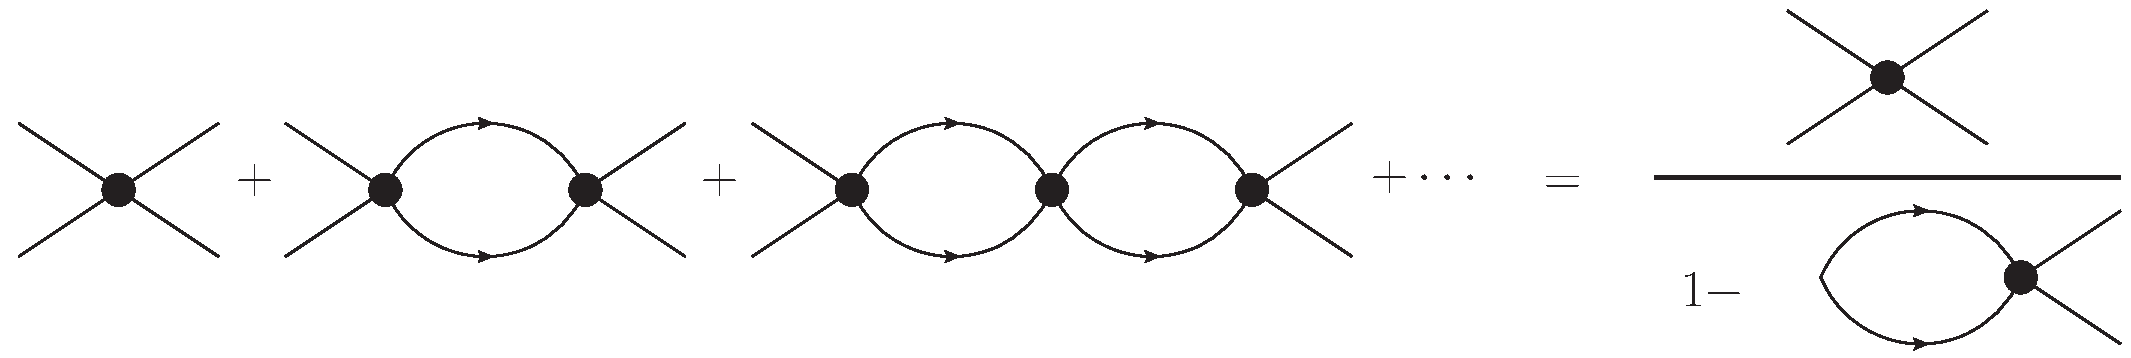
\includegraphics[width=.675\columnwidth]{figure/bubbleSum.pdf}
\hfill
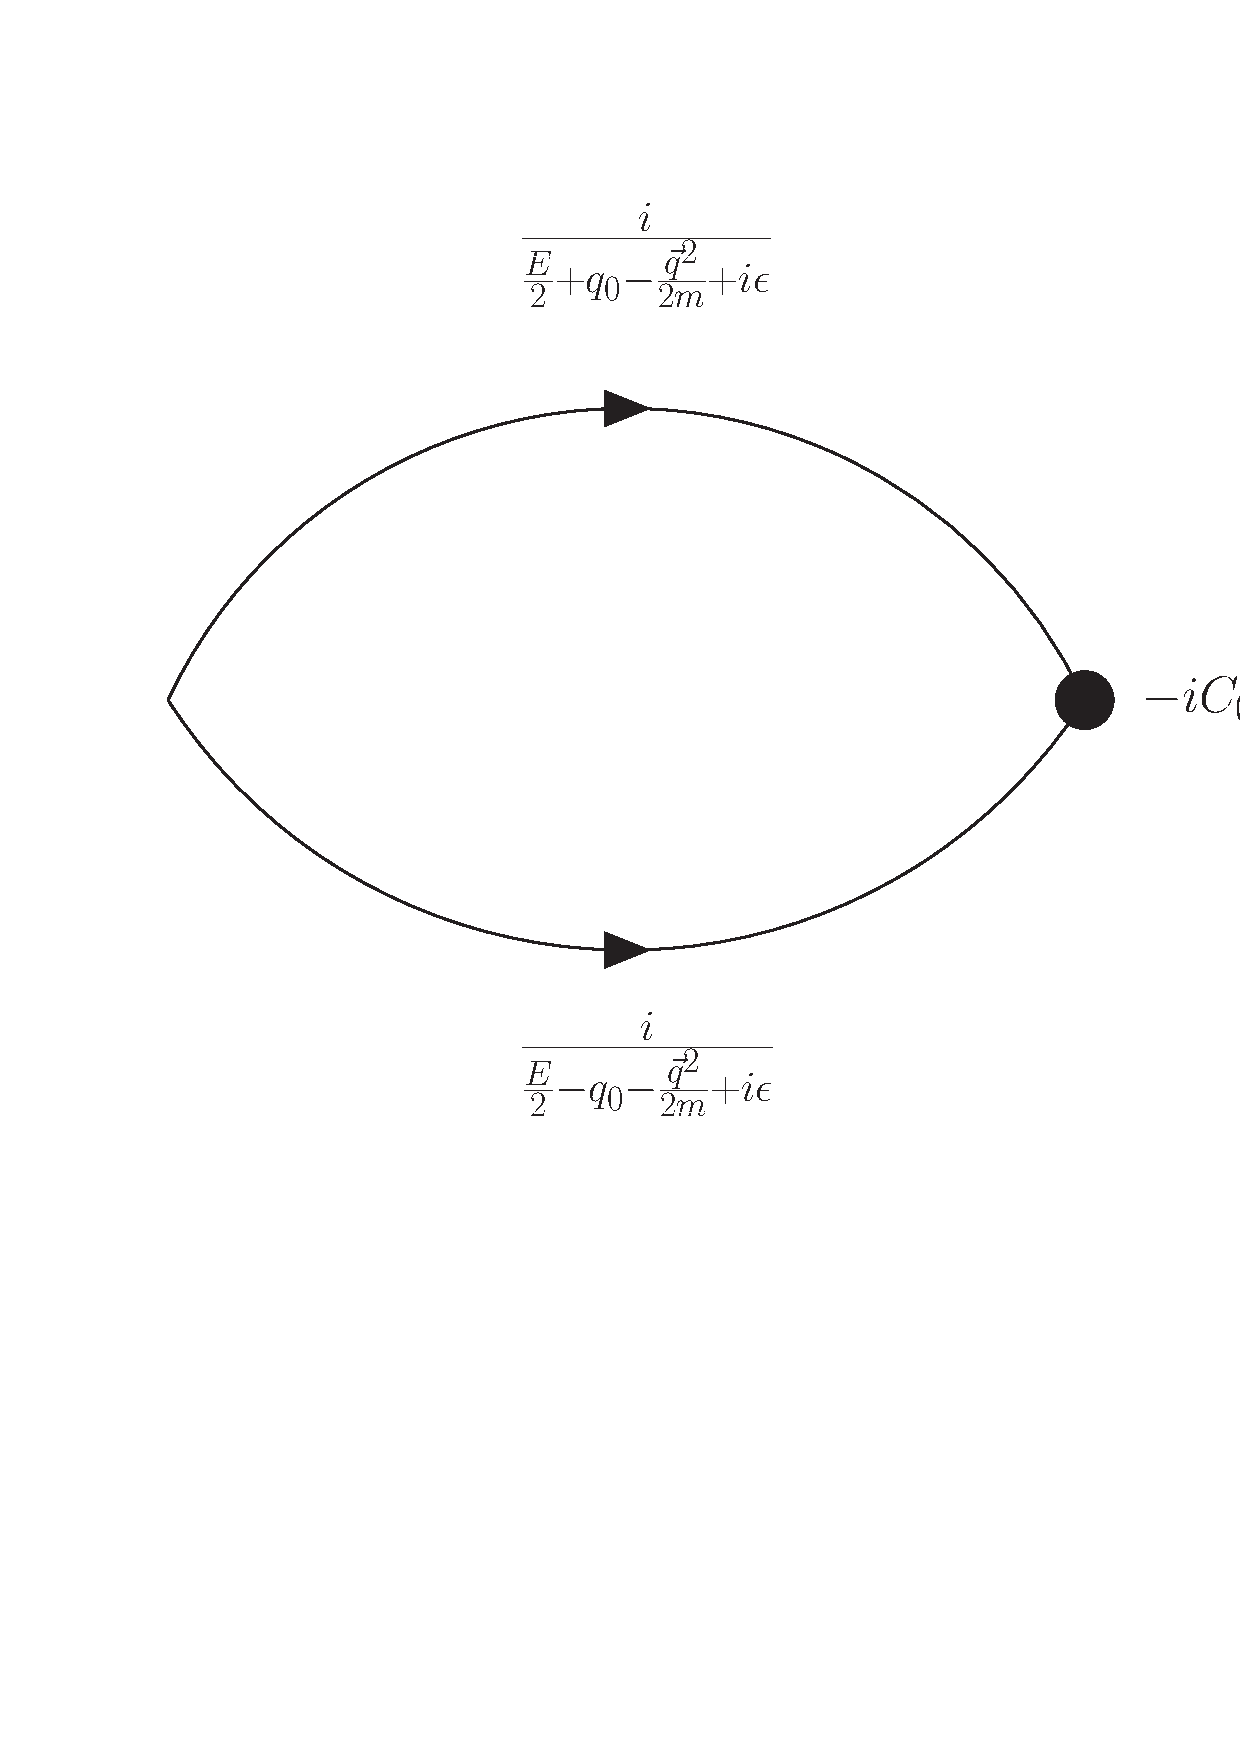
\includegraphics[width=.275\columnwidth]{figure/I0.pdf}
\caption{(Left) The bubble sum. Each line represents a propagator, each vertex represents $-i C(\Lambda)$, and the bubble is given by $I_D$.
(Right) The single loop diagram needed to calculate $I_D$ in the bubble sum.
\label{fig:bubbleSum}}
\end{figure}

This bubble sum is a geometric series and, restricting our attention to the contact interaction causes all other partial wave than the S-wave to vanish.
This restriction gives for the standard on-shell $T$-matrix
\begin{equation}\label{eq:T matrix}
T_{D\l}(p, \Lambda) = \delta_{\l 0} \frac{C(\Lambda)}{1-I_D(p,\Lambda) C(\Lambda)},
\end{equation}
where $p$ is the relative on-shell momentum, $\Lambda$ the regularization scale.
The physical result for the T-matrix is recovered once the parameter $C$ is chosen such that one can remove the regularization scale---in the limit of $\Lambda \to \infty$ for a hard momentum cutoff, for example.

$I_D(p,\Lambda)$ is a $D$-dependent function that arises from integrating the loop shown in the right panel of \Figref{bubbleSum},
\begin{align}
    I_D(p, \Lambda)
    &=-i\int^{\Lambda}
        \frac { \mathrm {d}q_0}{2\pi}\ \frac{\mathrm { d } ^ { D } \vec{ q } } { (2\pi)^ { D } }
        \left( \frac { i } { \frac{E}{2} + q _ { 0 } - \frac{\vec{q}^2}{2m_1} + i \epsilon } \right)
        \left( \frac { i } { \frac{E}{2} - q _ { 0 } - \frac{\vec{q}^2}{2m_2} + i \epsilon } \right)
    \label{eq:I0 in two particle language}\\
    &=\frac{\Omega_D}{(2\pi)^D}\int^{\Lambda}  \mathrm { d } q \ q^{D-1}\left[\PV \left( \frac { 1 } { E - \frac{\vec{q}^2}{2\mu} } \right)
-i\frac{\pi \mu}{q}\delta(q-\sqrt{2 \mu E})\right]
    \label{eq:I0 in relative coordinates}
    \\
    &=\frac{\Omega_D}{(2\pi)^2}\frac{2\mu}{L^{D-2}}\int^{\Lambda L/2\pi}  \mathrm { d } n \ n^{D-1}\left[\PV \left( \frac { 1 } { \left(\frac{pL}{2\pi}\right)^2 - n^2 } \right)
-i\frac{\pi^2}{L n}\delta\left(\frac{2\pi}{L}n -p\right)\right]
    \label{eq:I0}
\end{align}
where $\PV$ refers to Principal (Cauchy) Value, we have used the on-shell condition $2\mu E=p^2$, and the geometric factor
\begin{equation}
\Omega_D=\frac{2\pi^{D/2}}{\Gamma(D/2)}=
    \begin{cases}
    	2       &   (D=1)\\
		2\pi    &   (D=2)\\
        4\pi    &   (D=3)
    \end{cases}\ ,
\end{equation}
accounts for the angular integration in $D$ dimensions.

Because we are focusing on the contact interaction, we can restrict our attention to the $s$-wave, $\l=0$.
Dropping the $\l$ dependence in \eqref{on-shell-T}, the momentum-dependent $T$-matrix is related to the phase shift when
\begin{equation}\label{eq:spherical FD}
    \F_{D}(p)
    \equiv
    \begin{cases}
        p/2     & (D=1)\\
        1       & (D=2)\\
        \pi/p   & (D=3)\\
        \vdots  & \vdots
\end{cases}
\end{equation}
is a dimension-dependent kinematic factor determined by requiring the imaginary parts of the $T$-matrix \eqref{T matrix} from the bubble sum \eqref{I0 in relative coordinates} exactly matches the imaginary part of the amplitude \eqref{on-shell-T}.
This fixes the coefficients $C(\Lambda)$ as a function of the scattering data,
\begin{equation}\label{eq:IV pole}
    \frac{\mu}{2 \F_{D}(p)}\left(\cot \delta_{D}(p) - i\right)
    =
    \lim\limits_{\Lambda \to \infty} \left[ I_D(p, \Lambda) - \frac{1}{C(\Lambda)} \right].
\end{equation}

In a finite volume, the energy eigenstates $E$ appear at poles of the $T$-matrix, so that
\begin{equation}\label{eq:FV pole}
    \frac{1}{2\mu E C_\FV(\Lambda) } - I_{D, \FV}(\sqrt{2\mu E}, \Lambda) = 0
\end{equation}
and the infinite-volume integral $I_D$ has been replaced by the matching finite-volume sum which introduces another scale $L$,
\begin{align}
I_{D,\FV}(\sqrt{2\mu E}, \Lambda)
    &=-i\int \frac { \mathrm {d}q_0}{2\pi} \frac{1}{L^D}\sum_{\vec{q}}^{q < \Lambda} \left( \frac { i } { \frac{E}{2} + q _ { 0 } - \frac{\vec{q}^2}{2m_1} + i \epsilon } \right) \left( \frac { i } { \frac{E}{2} - q _ { 0 } - \frac{\vec{q}^2}{2m_2} + i \epsilon } \right)
    \\
    \label{eq:I0 FV}
    &=\frac{1}{L^D}\sum_{\vec{q}}^{q < \Lambda} \frac { 1 } { E - \frac{\vec{q}^2}{2\mu} }
    =\frac{2\mu}{(2\pi)^2 L^{D-2}} \sum_{\vec{n}}^{n < \frac{\Lambda L}{2\pi}} \frac{1}{x-n^2}
    &
    x &= \frac{2\mu E L^2}{4\pi^2}
    \, .
\end{align}
Combining the infinite-volume and finite-volume relations \eqref{IV pole} and \eqref{FV pole} yields
\begin{equation}\label{eq:spherical zeta}
    \frac{\mu}{2\F_{D}(\sqrt{2\mu E})}(\cot\delta_{D}(\sqrt{2\mu E})-i)
    =
    \lim\limits_{\Lambda \to \infty} \left[ I_D(\sqrt{2\mu E}) - I_{D,\FV}(\sqrt{2\mu E}) \right] \, ,
\end{equation}
the finite-volume quantization condition.
Note that both equations are explicitly evaluated for the same interactions $C_\FV(\Lambda) = C(\Lambda)$ independent of the volume $L$ and using the same regulator.
Furthermore \eqref{spherical zeta} is only valid if evaluated at momenta corresponding to finite-volume eigenenergies $E$.

Plugging our results for the integrals in, one finds
\begin{multline}
    \frac{1}{2\F_{D}(\sqrt{2\mu E})}\left(\cot \delta_{D}(\sqrt{2\mu E}) - i\right)
    =\\
    \frac{2}{(2\pi)^2 L^{D-2}}
    \lim\limits_{\Lambda \to \infty}
    \left[
    	\left(\mathcal{P}\int_{\vec{n}} - \sum_{\vec{n}}\right) \frac{1}{x-n^2} +
		\frac{-i \pi^2\Omega_D}{L} \int \mathrm{d}n\ n^{D-2} \delta\left(\frac{2\pi}{L}n - \sqrt{2\mu E}\right)
	\right]
\end{multline}
where both the sum and integral are cut off by a restriction on the magnitude of $n$, $n^2 < (\Lambda L / 2\pi)^2$,
The principle value integration implicitly carries a factor of $\Omega_D n^{D-1}$ (see \eqref{I0}).
The imaginary part on the left hand side exactly cancels the last term on the right when $E\ge0$.  When $E<0$ the last term on the RHS vanishes and so we have
%--demanding this cancellation is how the kinematic factor $\F_D$ of the $T$ matrix is determined----and we are left with
\begin{multline}\label{eq:general luscher}
   \frac{1}{2\F_{D}(\sqrt{2\mu E})}  \left( \cot \delta_{D}(p)-i\theta(-E)\right)
    =
   \frac{2}{(2\pi)^2 L^{D-2}}
    \lim\limits_{\Lambda \to \infty}\left(\sum_{\vec{n}}-\mathcal{P}\int_{\vec{n}}\right) \frac{1}{n^2-x}\\
    \implies
      \cot \delta_{D}(p)= \frac{\F_{D}(\sqrt{2\mu E})}{\pi^2 L^{D-2}}\left[
    \lim\limits_{\Lambda \to \infty}\left(\sum_{\vec{n}}-\mathcal{P}\int_{\vec{n}}\right) \frac{1}{n^2-x}\right]
    +i\theta(-x)
    \ ,
\end{multline}
with $x$ as in \eqref{I0 FV}, $\theta(x)$ is the heavyside function, and we switched the sign of the sum and integral as well as the sign of the denominator.  In the second line above we moved the term proportional to the $\theta(-E)$ to the RHS.
Because we cut off the sum and the integral in exactly the same way, in dimensions where $I_D$ diverges with $\Lambda$, the divergence cancels against the divergence in the sum.
Let $N=\Lambda L/\pi$.
Then, with a finite cutoff on magnitude $N/2$, we define
\begin{equation}\label{eq:spherical cutoff S}
    S^{\spherical N}_D(x) =
    \left(\sum_{\vec{n}}- \mathcal{P}\int_{\vec{n}}\right) \frac{1}{n^2-x}
    + i \frac{(2\pi)^D}{4 \F_D\left(\sqrt{x}\right)}\theta(-x)\ ,
\end{equation}
where it was used that $\F_D(p) \sim p^{2-D}$ and the $\spherical$ superscript reminds us that we cut off our sum and integral in a spherical way, based on the magnitude of $n<N/2$.   By performing the principal value integral and taking the limit $N\to \infty$, we recover the usual \Luscher zeta functions,
\begin{equation}\label{eq:spherical S}
    S^\spherical_D(x)
    =
    \lim_{N\goesto\infty} S^{\spherical N}_D(x)
    =
    \lim_{N\rightarrow\infty} \sum_{\vec{n}}^{n < N/2}
    \begin{cases}
     \frac{1}{n^2-x} - \counterterm_3^\spherical \frac{N}{2}& (D=3)\\
     \frac{1}{n^2-x} - 2\pi\log\left(\counterterm_2^\spherical\frac{N}{2}x^{-1/2}\right)& (D=2)\\
    \frac{1}{n^2-x} & (D=1)
     \end{cases}
\end{equation}
where the dimension-dependent coefficients $\counterterm_D^\spherical$ of the counterterms come from the principal value integral; we evaluate the spherical-cutoff integrals and extract these coefficients in \Appref{counterterm/spherical}.\footnote{In higher dimensions there will be additional divergences which cancel, for example, in five spatial dimensions there will be a cubic and linear divergence.
}
Finally, we can write the quantization condition~\eqref{general luscher} using the zeta function~\eqref{spherical S},
\begin{equation}\label{eq:spherical quantization}
    \cot \delta_{D}(p) = \frac{\F_{D}(p)}{\pi^2 L^{D-2}} S^\spherical_D(x)
\end{equation}
where we traded the energy dependence for momentum on the left-hand side.  Our result is consistent with those given in~\Ref{Zhu:2019dho}\footnote{In~\Ref{Zhu:2019dho} the zeta functions~\eqref{spherical cutoff S} were defined \emph{without} the term proportional to the heavyside function.  Thus their zeta functions have a different behavior for $x<0$ as ours.  We note that our definition is more common in the literature.}.
This is the \Luscher finite-volume quantization condition, and finite-volume energy levels calculated in the continuum should be fed through it to produce continuum scattering data.
In three dimensions it is common to move the momentum dependence in $\F_{D}$ to the other side, as $p \cot\delta_{D}(p)$ is what appears in the effective range expansion \eqref{ere}.
In two dimensions, it will prove useful to explicitly separate the logarithmic divergence as $N\to\infty$ from the logarithmic singularity as $x\to 0$, and we will rearrange this equation and slightly redefine $S^\spherical_2$ as needed in \Secref{2D}.  Finally, the sum in~\eqref{spherical S} can be analytically done in $D=1$, as we will show in \Secref{1D}.

%Derived in the zero-temperature continuum, only cold continuum-extrapolated spectra ought to be fed through the quantization condition \eqref{spherical quantization} to extract continuum phase shifts.

To approach the continuum limit, the authors of \Ref{Lee:2007ae} proposed tuning the interaction until the ground state, when fed through $S^\spherical$, produced the desired amplitude that corresponds to the desired scattering length.
We will show in \Secref{3D} that this procedure induces a momentum dependence in the scattering amplitude sensitive to discretization.
In the next subsection we give a procedure that produces a momentum-independent amplitude as one approaches the continuum, and discuss the limiting procedure itself.

\section{The Dispersion \Luscher Finite-Volume Counterterm}\label{sec:counterterm/dispersion}

To evaluate the infinite-volume integral in \eqref{dispersion S},
\begin{equation}
    \left(\frac{N}{2}\right)^{D-2}
    4\pi^2 \int_{-N/2}^{+N/2} \mathrm{d}^Dn\; \PV \frac{1}{N^2 \sum_{ds} \gamma^{(\nstep)}_s \cos \frac{2\pi n_d s}{N} - x}
    =
    4\pi^2 \left(\frac{N}{2}\right) \int_{-1}^{+1} \mathrm{d}^D\nu\; \PV \frac{1}{4\sum_{ds} \gamma^{(\nstep)}_s \cos \pi \nu s - \tilde{x}}
\end{equation}
where as in the Cartesian case we rescaled and $\tilde{x} = x/(N/2)^2$.
Note that when we replace the sum over dimensions and steps with the exact $p^2$ result $(\pi \nu)^2$ and let $\tilde{x}$ vanish, we can match \eqref{cartesian S counterterm}.

We can use the same trick to isolate the leading behavior in $N/2$, introducing the dispersion relation in the exponent rather than $n^2$.
One finds a coefficient multiplying $(N/2)^{D-2}$,
\begin{equation}
    \label{eq:dispersion counterterm}
    \mathcal{L}^{\dispersion (\nstep)}_D = 4 \pi^2 \int_{0}^{\infty} 2\mu\; \mathrm{d}\mu\; \left(\int_{-1}^{+1} \mathrm{d}\nu\; e^{-4\mu^2 \sum_s \gamma_s^{(\nstep)} \cos \pi \nu s}\right)^D
\end{equation}
which can be numerically evaluated quickly, assuming one has the dispersion relation coefficients in hand.
In \Figref{nstep counterterm} we show this counterterm and how it differs from the $\nstep=\infty$ counterterm.

\begin{figure}
    \includegraphics{figure/counterterm-nstep.pdf}
    \caption{In the top panel we show the dispersion counterterm $\mathcal{L}^{\dispersion (\nstep)}_{3}$in \eqref{dispersion counterterm} as a function of $\nstep$, and the $\nstep=\infty$ result, which is the same as the Cartesian result $\mathcal{L}^{\cartesian}_3$, as a dashed line.  In the bottom panel we show a better view into how the counterterm converges to the Cartesian one.
    }
    \label{fig:nstep counterterm}
\end{figure}

